\documentclass{article}
\usepackage{graphicx} % Required for inserting images
\usepackage{amsmath}
%\usepackage{subfigure}
\usepackage{subcaption}
\usepackage{amsfonts}
\usepackage{mdframed}
\usepackage{xcolor}
\usepackage{hyperref}


\usepackage[left=2cm, right=2cm, top=2cm, bottom=2cm]{geometry}

\setlength{\parindent}{0pt}

\definecolor{LightGray}{gray}{0.95}

\title{Data and Observer Design -- Final Project}
\author{Esraaj Sarkar Gupta, Manan Gadesha, Kanishk Khandelwal}
\date{March 2026}

\begin{document}

\maketitle

\section{Introduction}
In this project, an IMU is programmed with a number of algorithms to estimate the orientation of the IMU.

\begin{enumerate}
    \item Pure Gyroscope Integration
    \item Tri-axial Attitude Determination (TRAIDS)
    \item Explicit Mahony Filter
    \item Direct Complimentary Filter
    \item Passive Complimentary Filter
\end{enumerate}

\textbf{If you are evaluating this report for grading, skip to Section 3 for Calibration Logic and Section 4 for Observations and Results.}\\
\\
This paper begins by exploring the mathematical representation of these algorithms, and follows up with the calibration logic used to calibrate the sensors (Accelerometer, Gyroscope and Magnetometer) onboard the IMU, and finally reports on the observations from each algorithm.\\
\\
All the programs and some of the data used in this project are all available on the \href{https://github.com/Esraaj-Sarkar-Gupta/Observer-Design}{Project Github Repository}.

\section{Mathematical Background}
In this project, two frames of reference have been considered. The primary frames are the
\begin{enumerate}
    \item \textbf{The Inertial Reference Frame} $\mathcal{I}$ is a fixed, world aligned frame. This implementation uses a modified ENU (East, North, Up) convention where the reference gravity points directly downwards $r_g = [0,0,-1]^T$ and True North points along the Y-axis $r_N = [0, 1, 0]^T$.
    \item \textbf{The Body Frame} $\mathcal{B}$ is the local coordinate frame rigidly attached to the IMU sensor.
\end{enumerate}

To map angular velocities from $\mathbb{R}^3$ into the Lie algebra $\mathfrak{so}(3)$, we define the skew-symmetric operator $(\cdot)^\times$. For an angular velocity vector $\Omega = [\omega_x, \omega_y, \omega_z]^T$:
\begin{equation}
   \Omega^\times = \begin{bmatrix} 0 & -\omega_z & \omega_y \\ \omega_z & 0 & -\omega_x \\ -\omega_y & \omega_x & 0 \end{bmatrix}
\end{equation}

\subsection{Pure Gyroscope Rotation on $SO(3)$}

The fundamental kinematic equation governing the rotation of a rigid body subject to an angular velocity $\Omega$ is:
\begin{equation}
    \dot{R} = R \Omega^\times
\end{equation}

\[
\]

To implement this in a discrete-time digital system with a sample time $\Delta t$, the matrix exponential is utilized to advance the rotation matrix forward in time:
\[
R_{k+1} = R_k \exp(\Omega^\times \Delta t)
\]

Computing a true matrix exponential is computationally expensive. Because $\Omega^\times$ belongs to $\mathfrak{so}(3)$, the exponential map can be solved exactly using \textbf{Rodrigues' Rotation Formula}. By defining the magnitude of rotation $\theta = ||\Omega||\Delta t$ and the normalized axis of rotation $K = \frac{\Omega^\times}{||\Omega||}$, the integration becomes:
\[
\exp(\Omega^\times \Delta t) = I_3 + \sin(\theta)K + (1 - \cos(\theta))K^2
\]

While this method provides an exact local update, pure open-loop integration accumulates unbounded error over time due to gyroscope noise and bias.

\subsection{Tri-Axial Attidue Determination (TRIAD Estimation)}
\
TRIAD is a deterministic, algebraic method that constructs a full rotation matrix from two non-parallel vector measurements. In this framework, it uses the normalized accelerometer reading ($v_1$) and magnetometer reading ($v_2$). 

TRIAD enforces a strict hierarchy, designating the accelerometer as the absolute truth for pitch and roll, while using the magnetometer solely to resolve the yaw (heading). An orthogonal basis is constructed in the Body Frame ($\mathcal{B}$):
\begin{align*}
t_1 &= v_1 \\
t_2 &= \frac{t_1 \times v_2}{||t_1 \times v_2||} \\
t_3 &= t_1 \times t_2
\end{align*}

A corresponding orthogonal basis is constructed in the Inertial Frame ($\mathcal{I}$) using the ideal reference vectors for gravity ($r_1$) and North ($r_2$):
\begin{align*}
\hat{r}_2 &= \frac{r_1 \times r_2}{||r_1 \times r_2||} \\
r_3 &= r_1 \times \hat{r}_2
\end{align*}

By concatenating these basis vectors into matrices $W_\mathcal{B} = [t_1, t_2, t_3]$ and $W_\mathcal{I} = [r_1, \hat{r}_2, r_3]$, the rotation matrix is calculated directly:
\begin{equation}
    R_{triad} = W_\mathcal{I} W_\mathcal{B}^T
\end{equation}

It must be noted that this algorithm fundamentally breaks down if gravity is perfectly perpendicular to True North $v_1 \perp v_2$, given that in this case the cross product for $v_1 \times v_2$ vanishes. This causes a division-by-zero error when computing $t_2$.

\subsection{Explicit Complementary Filter (Mahony)}

The Mahony filter is a nonlinear observer that operates directly on the $SO(3)$ manifold. Unlike TRIAD, which calculates attitude statically, the Explicit filter integrates the gyroscope data while applying continuous feedback correction based on vector discrepancies.\\
\\
The filter rotates the ideal inertial reference vectors into the estimated Body Frame using the transpose of the current estimate ($\hat{R}^T$). The measured magnetic field is rotated into the inertial frame ($h = \hat{R}v_2$), and a synthetic reference vector $b$ is generated that forces East to zero, places the full horizontal magnitude into North, but preserves the measured vertical plunge ($h_z$):

\begin{equation}
   b = \bigg[0, \sqrt{h_x^2 + h_y^2}, h_z \bigg]^T 
\end{equation}

The Body-Frame estimates are thus:

\begin{equation}
   \hat{v}_a = \hat{R}^T r_1 \quad \text{and} \quad \hat{v}_m = \hat{R}^T b
\end{equation}

The angular error $e$ is the sum of the cross products between the physical measurements and these estimates:

\begin{equation}
    e = (v_1 \times \hat{v}_a) + (v_2 \times \hat{v}_m)
\end{equation}

This error vector drives a Proportional-Integral (PI) controller, yielding a corrected angular velocity that replaces the raw gyroscope data in Rodrigues' formula:

\begin{equation}
    \Omega_{corr} = \Omega_{raw} + K_p e + K_i \int e \, dt
\end{equation}

\subsection{Direct Complementary Filter}

The Direct Complementary Filter is similar in architecture to the Explicit filter, but instead of computing error from raw vector cross-products, it utilizes the complete rotation matrix generated by the TRIAD algorithm ($R_{triad}$) as a direct measurement reference.\\
\\
The rotational error is computed as the difference between the current estimate $\hat{R}$ and the TRIAD measurement, calculated within the Body Frame:
\begin{equation}
\tilde{R} = \hat{R}^T R_{triad}
\end{equation}

To extract a 3D correction vector from this matrix difference, the skew-symmetric component is isolated and vectorized using the $\text{vex}(\cdot)$ operator:
\begin{equation}
e_{direct} = \text{vex} \left( \frac{\tilde{R} - \tilde{R}^T}{2} \right)
\end{equation}

\begin{mdframed}[backgroundcolor=gray!10]
    \textbf{The Vex Operator}\\
    In the context of Lie groups and Lie algebras, mapping between a 3D vector and its corresponding $3 \times 3$ skew-symmetric matrix is carried out by the vex operator. While the $(\cdot)^\times$ operator maps a vector $v \in \mathbb{R}^3$ to a skew-symmetric matrix $S \in \mathfrak{so}(3)$, the \textbf{vex} operator performs the exact inverse operation.

    Given a $3 \times 3$ skew-symmetric matrix $S$ defined as:
    \begin{equation}
    S = 
    \begin{bmatrix} 
    0 & -v_z & v_y \\ 
    v_z & 0 & -v_x \\ 
    -v_y & v_x & 0 
    \end{bmatrix}
    \end{equation}
    
    The $\text{vex}(\cdot)$ operator extracts the independent components to reconstruct the original 3D vector:
    \begin{equation}
    \text{vex}(S) = 
    \begin{bmatrix} 
    v_x \\ 
    v_y \\ 
    v_z 
    \end{bmatrix}
    \end{equation}
\end{mdframed}

This body-frame error vector is then routed through the standard PI controller ($\Omega_{corr} = \Omega_{raw} + K_p e_{direct} + \dots$) and integrated to update the state.

\subsection{Passive Complementary Filter}

The Passive Complementary Filter is designed to guarantee passivity, a control systems property ensuring that the estimation error naturally dissipates energy, guaranteeing bounded stability.\\
\\
To achieve this, the rotational difference is computed in the Inertial Frame rather than the Body Frame:
\begin{align*}
\tilde{R}_{inertial} &= R_{triad} \hat{R}^T \\
e_{inertial} &= \text{vex} \left( \frac{\tilde{R}_{inertial} - \tilde{R}_{inertial}^T}{2} \right)
\end{align*}

Because the necessary correction must be applied to the gyroscope (which generates data natively in the Body Frame), this inertial error must be rotated back down into the local coordinate system before it can be used:
\begin{equation}
e_{body} = \hat{R}^T e_{inertial}
\end{equation}

Once rotated, the error is processed by the PI controller and integrated just as in the Direct and Explicit filters, yielding a highly stable, drift-free orientation estimate.

\section{Sensor Calibration}
The IMU sensors are calibrated in for both steady state systemic biases, and dynamic systemic biases.

\subsection{Steady State Biases}
The steady state biases for the accelerometer and gyroscope are calibrated against.

\begin{figure}[htbp]
     \centering
     \begin{subfigure}[b]{0.45\textwidth}
         \centering
         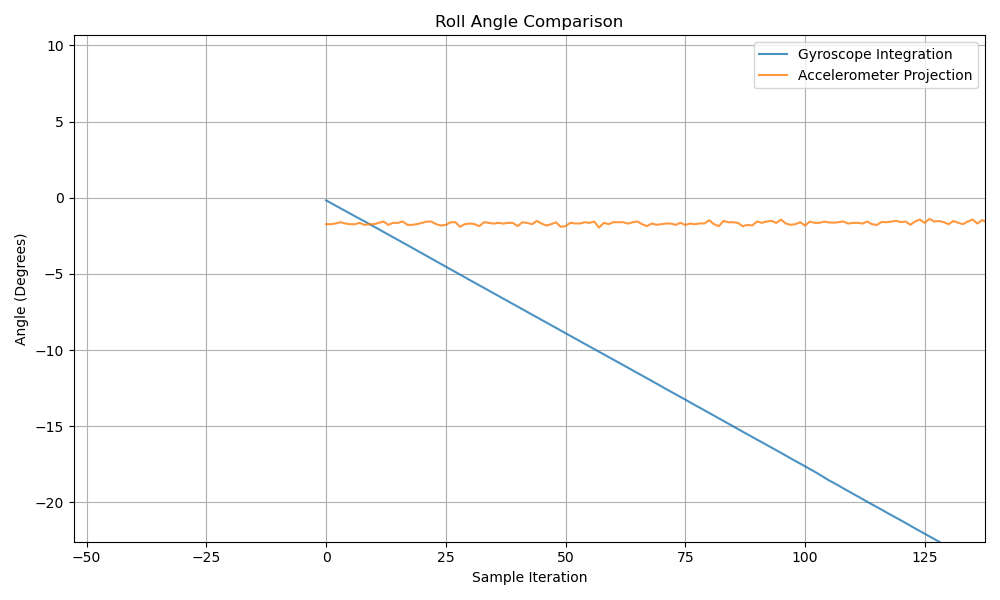
\includegraphics[width=\textwidth]{systemic_bias.png}
         \caption{Bias in Device Measurements}
         \label{fig:systemic_bias}
     \end{subfigure}
     \hfill
     \begin{subfigure}[b]{0.45\textwidth}
         \centering
         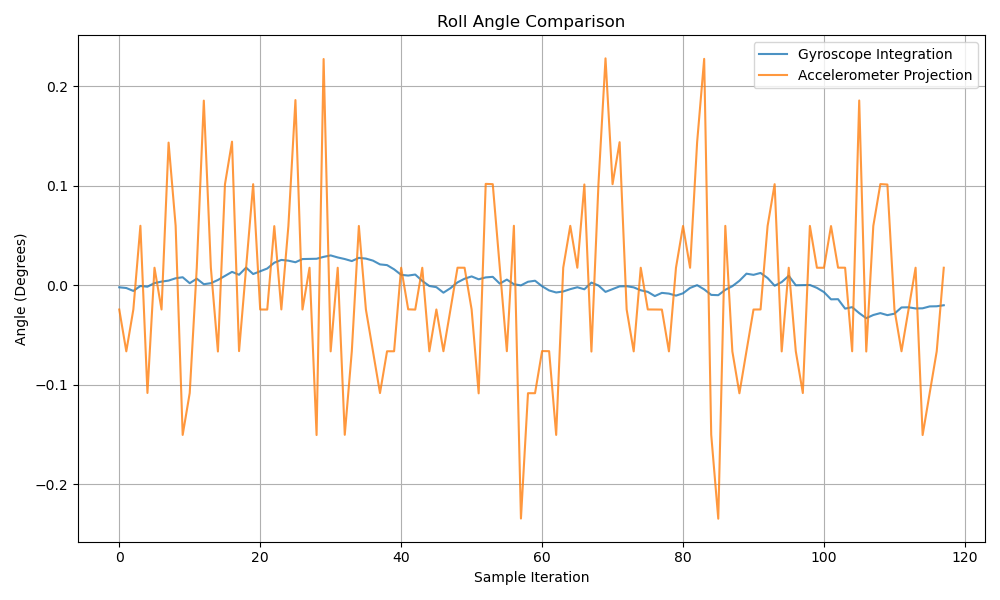
\includegraphics[width=\textwidth]{bias_correction.png}
         \caption{}
         \label{fig:bias_correction}
     \end{subfigure}
        \caption{Errors in Device Measurements}
        \label{fig:errors}
\end{figure}

This error is corrected for by including a "burn-in" period, during which the device is allowed to rest. Measurements from the idle device are averaged for all columns and subtracted with the expected values (all zero apart from $a_z$). The bias for each column is subsequently subtracted from every reading during the "main" cycle following the burn-in cycles. It is evident from Fig.\ref{fig:bias_correction} that this is effective.\\
\\
One may still observe aliasing if the device is perturbed faster than its Nyquist Limit. This is demonstrated in Fig. \ref{fig:aliasing}.

\begin{figure}[h!]
    \centering
    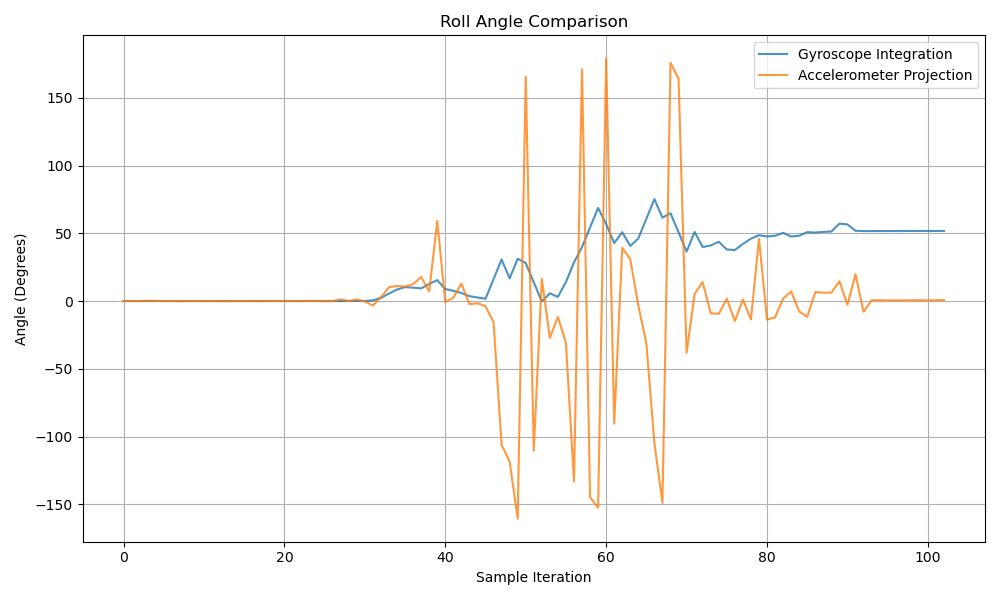
\includegraphics[width=0.5\linewidth]{errors_compound.png}
    \caption{Aliasing}
    \label{fig:aliasing}
\end{figure}

The steady-state errors recorded on the hardware have been given in Fig. \ref{fig:gyc_acc_errors}.

\begin{figure}[h!]
    \centering
    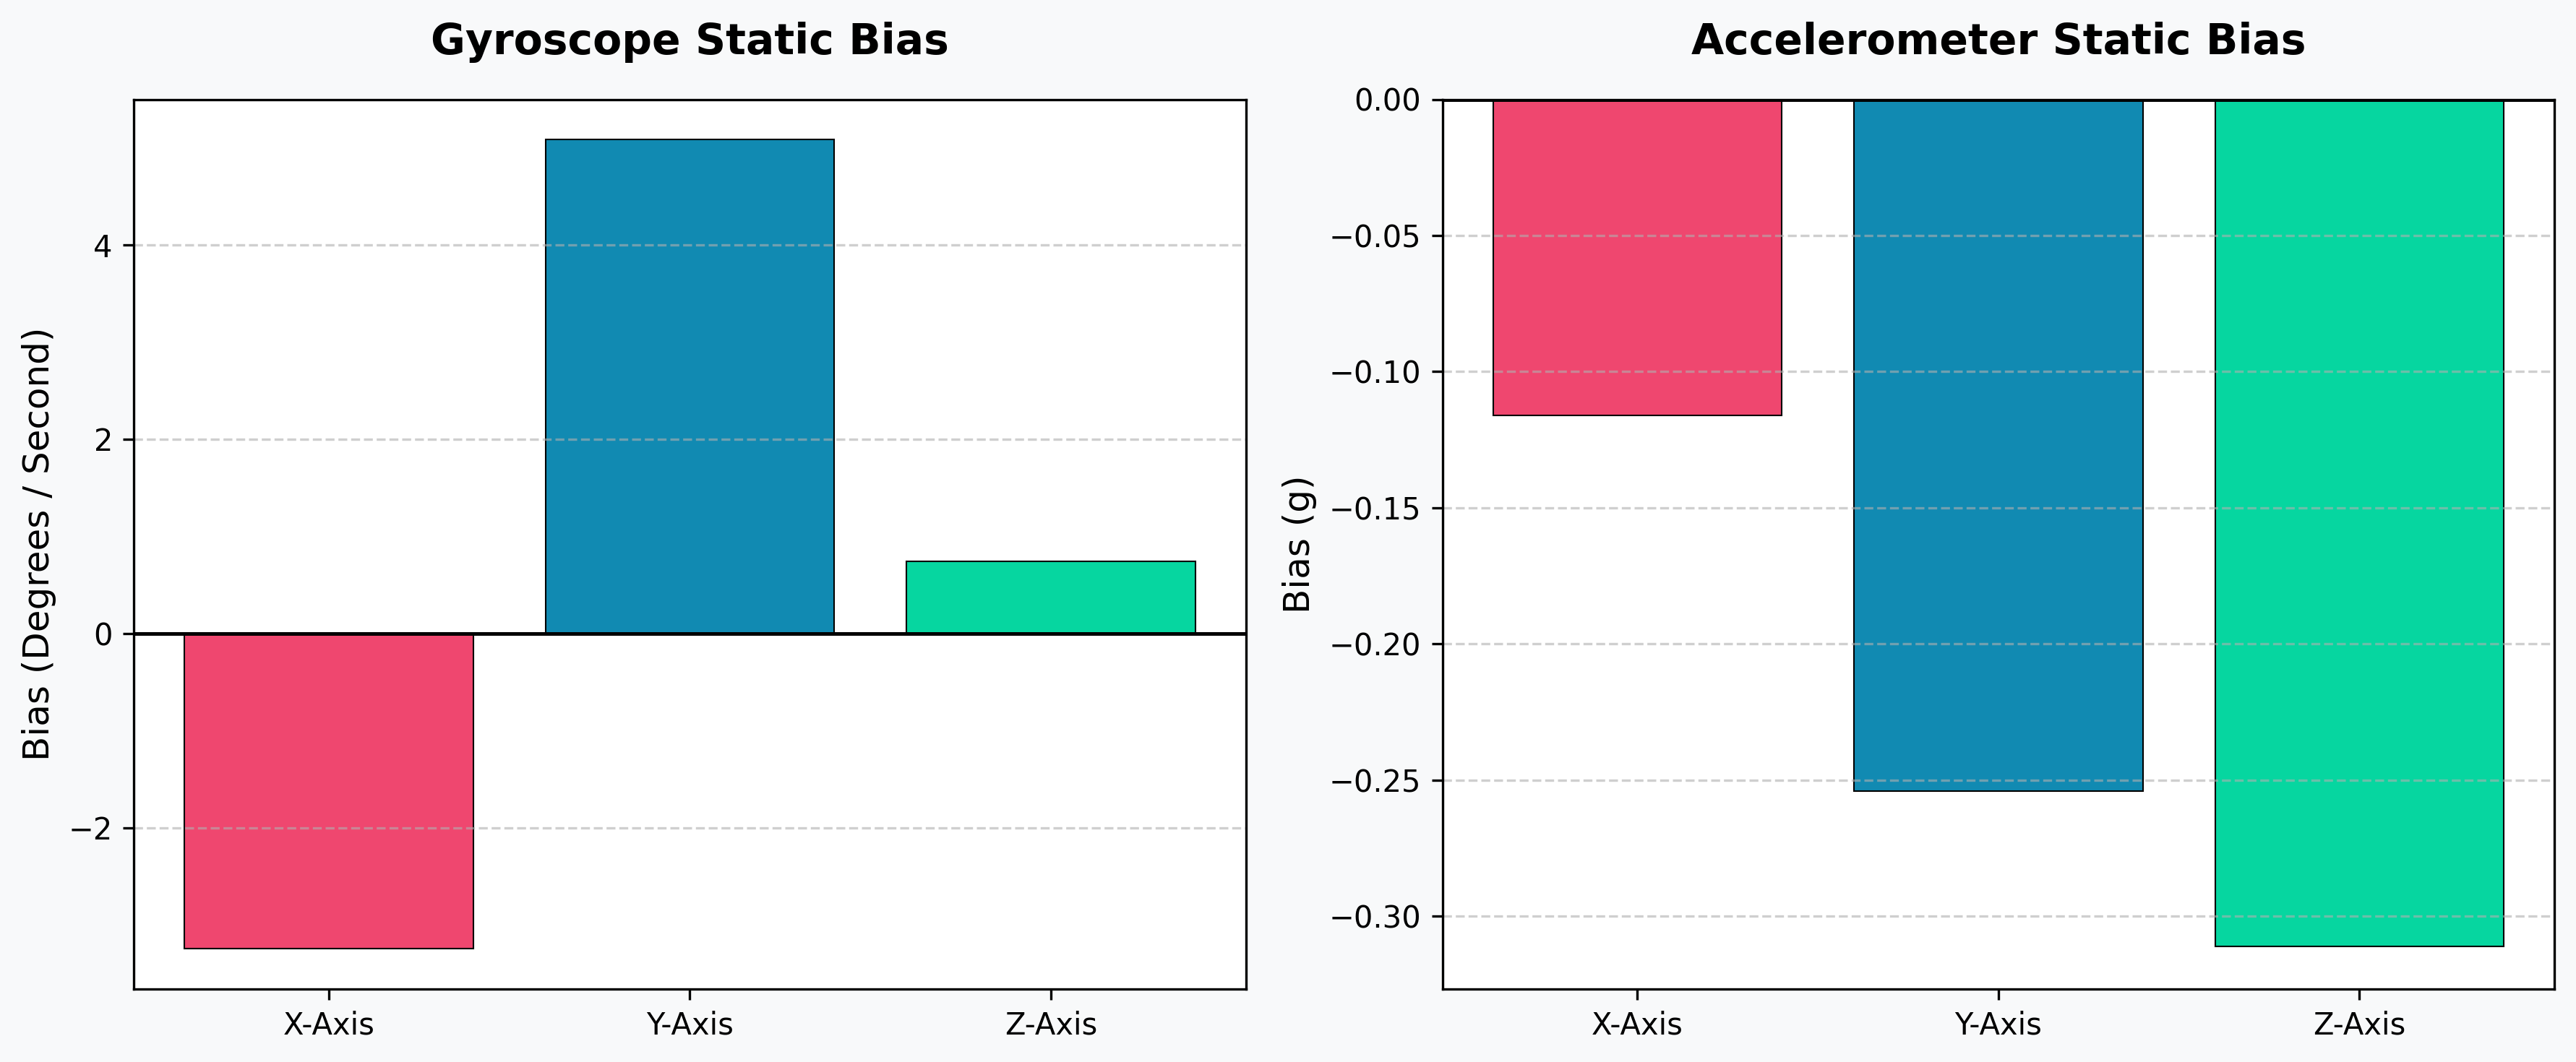
\includegraphics[width=0.8\linewidth]{gyro_acc_barcharts.png}
    \caption{Gyroscope and Accelerometer Steady-State Errors}
    \label{fig:gyc_acc_errors}
\end{figure}

\subsection{Magnetometer Static + Dynamic Errors}
The biases in magnetometer measurements fall into the categories \textbf{Hard Iron Errors} and \textbf{Soft Iron Errors}.

\begin{enumerate}
    \item \textbf{Hard Iron Errors: } Caused by materials that have an intrinsic magnetic field.

    \begin{equation}
        v_\text{measured} = v_\text{true} + b_\text{hard}
    \end{equation}
    
    \item \textbf{Soft Iron Errors: } Caused by materials with high magnetic permability.
\end{enumerate}

All biases are represented as a linear transformation $W_{3\times3}$ of the true magnetic vector.

\begin{equation}
    V_\text{measured} = Wv_\text{true}
\end{equation}

Taking the sensor through all possible configurations and plotting the results of all the vectors $v$ (ideally) results in a sphere, given by $v_\text{true}^T v_\text{true} = r^2$. From the measurements made, this expression is given by

\begin{equation}
    \big(W^{-1}v_\text{measured}\big)^T\big(W^{-1}v_\text{measured}\big) = r^2
\end{equation}

yielding an ellipsoid with the expression 

\begin{equation}
    \big(v_\text{measured}\big)^TA \big( v_\text{measured} \big) = r^2
\end{equation}

where $A = \big(W^{-1}\big)^T W^{-1}$.

\begin{figure}
    \centering
    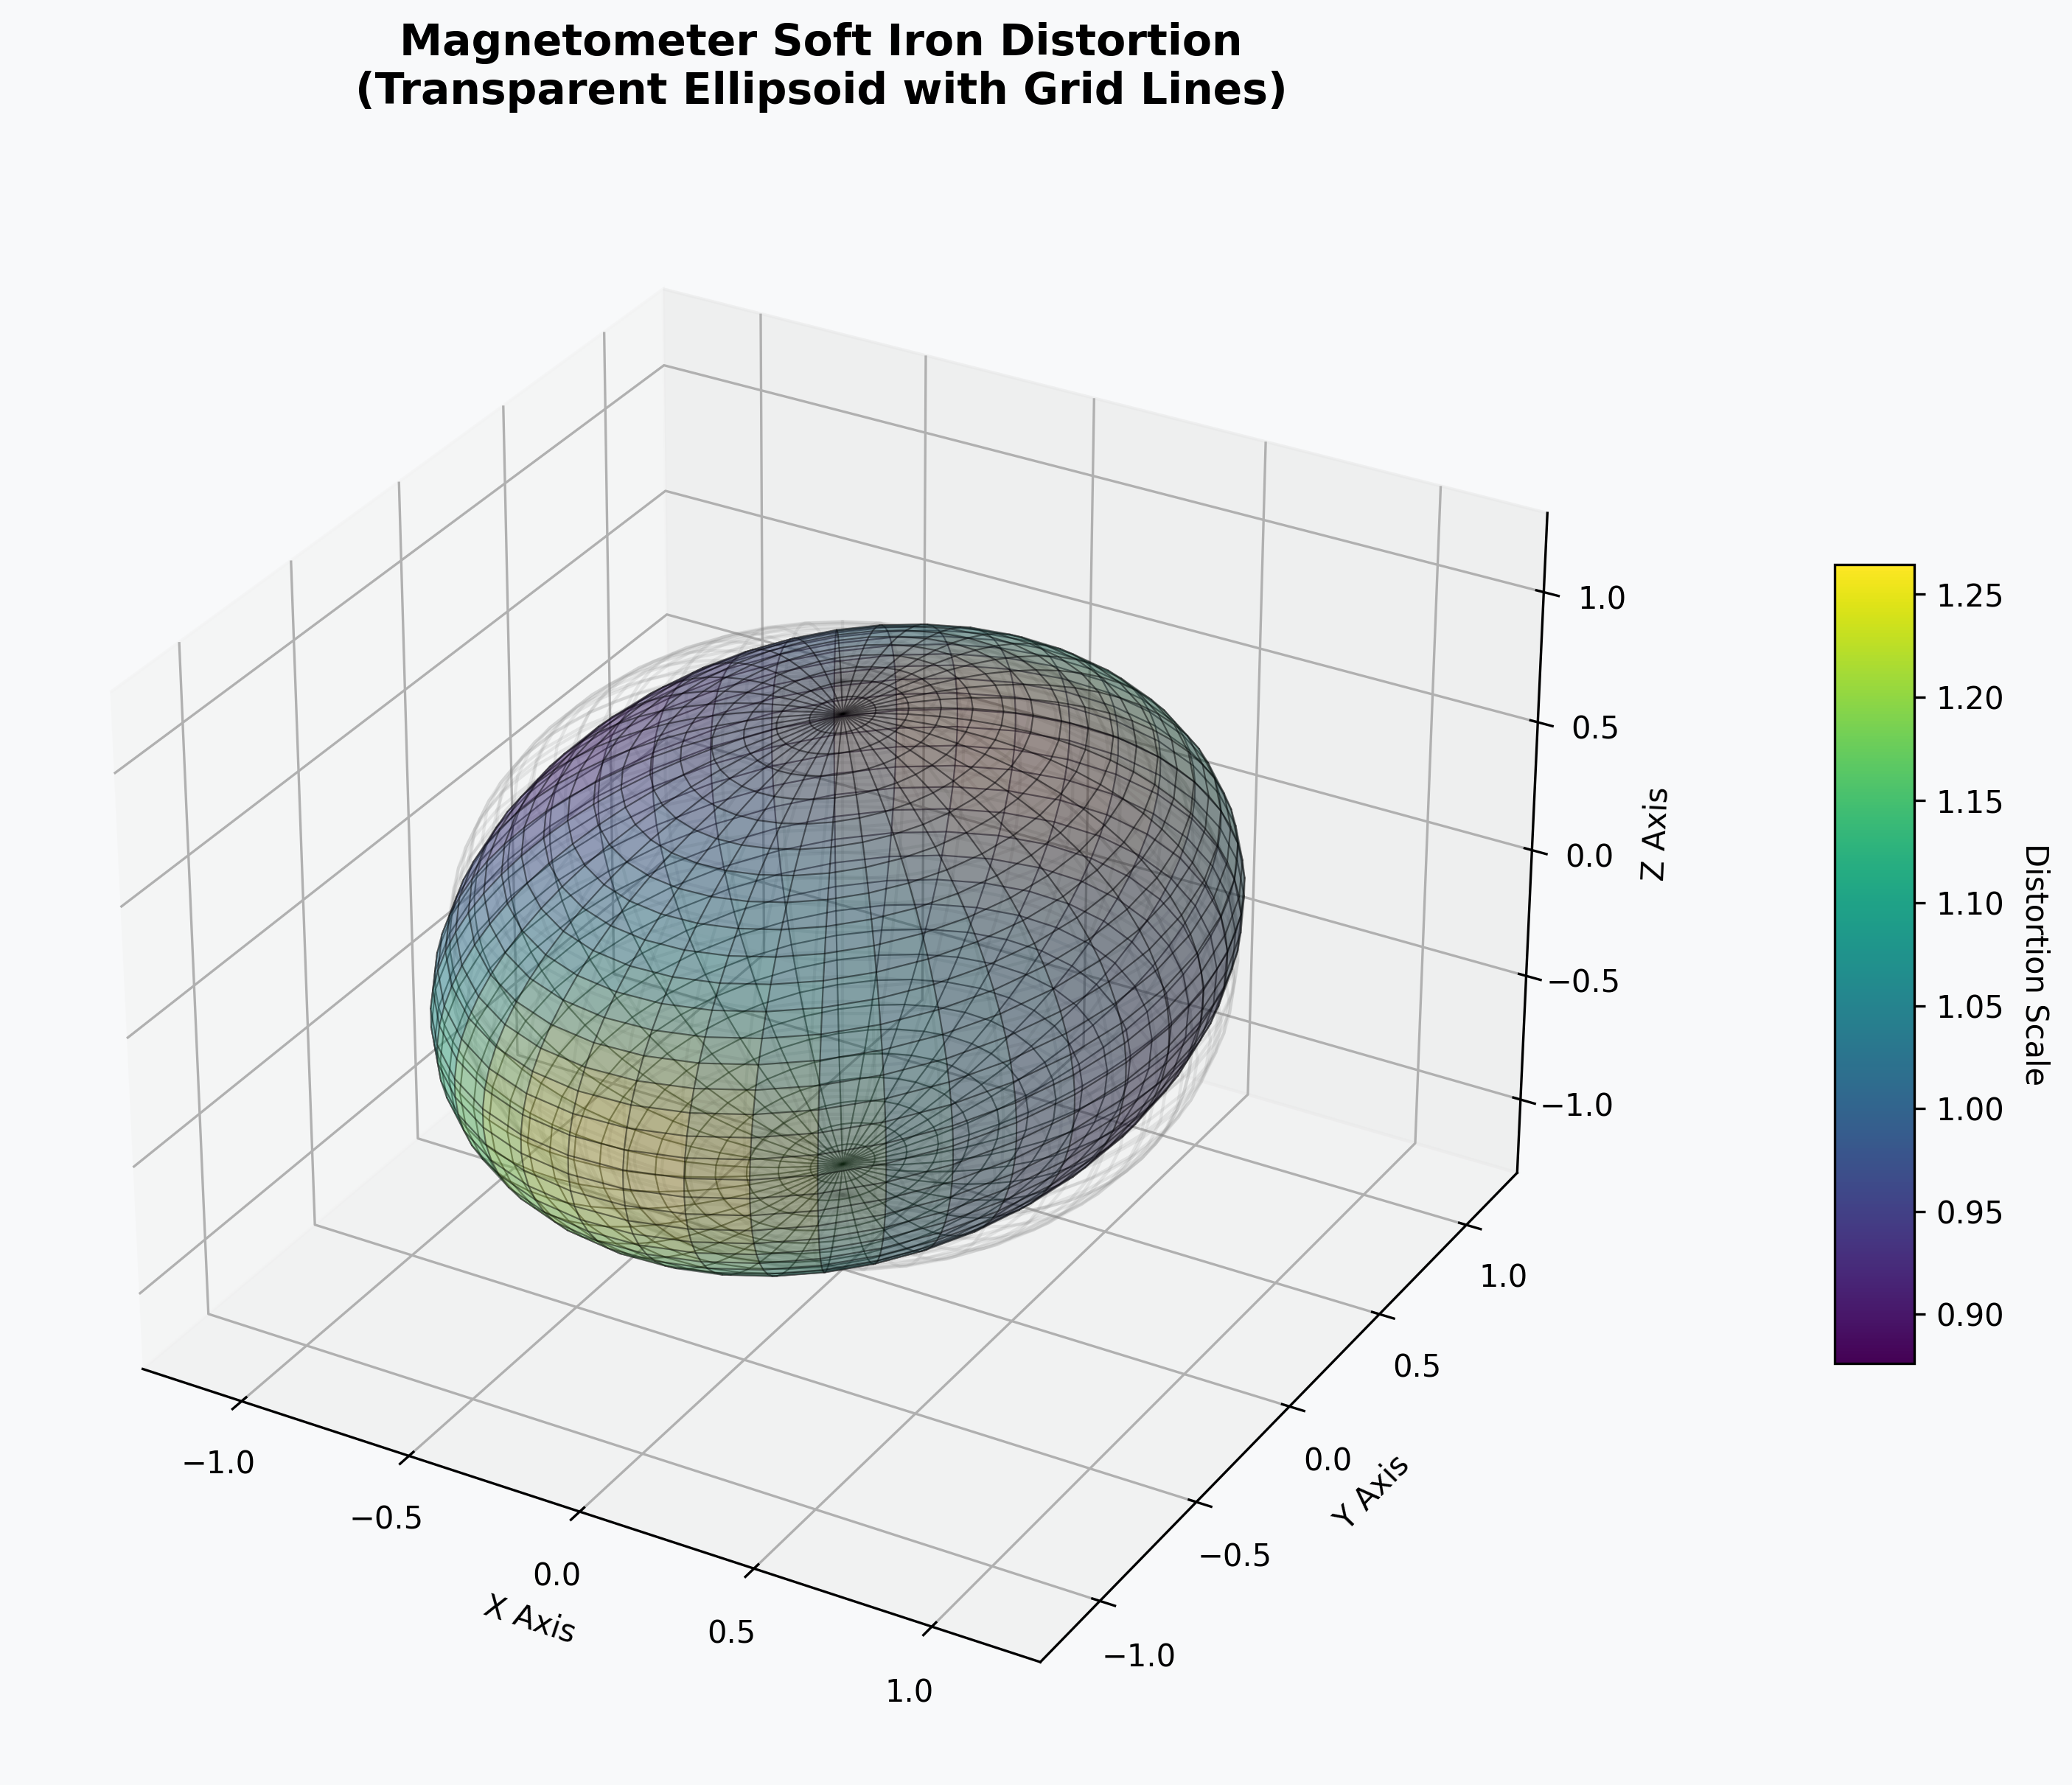
\includegraphics[width=0.5\linewidth]{mag_soft_iron_ellipsoid_transparent.png}
    \caption{Magnetic Vectors -- Ellipsoid}
    \label{fig:placeholder}
\end{figure}

In practice, one may compute $W$ by first computing the hard iron bias for each physical coordinate $X = x, y, z$.

\begin{equation}
    b_X = \frac{X_{\max} - X_{\min}}{2}
\end{equation}

Under the assumption that all soft-iron distortions occur along the basis of the magnetometer, the transformation matrix can be represented as a diagonal matrix. This assumption was chosen to keep computational overhead to a minimum allowing the processor to operate at greater speeds.\\
\\
Additionally, cross-coupling matrices were examined to have very small shear terms. Under these circumstances, it might be prudent to operate with diagonal matrices.

\begin{figure}
    \centering
    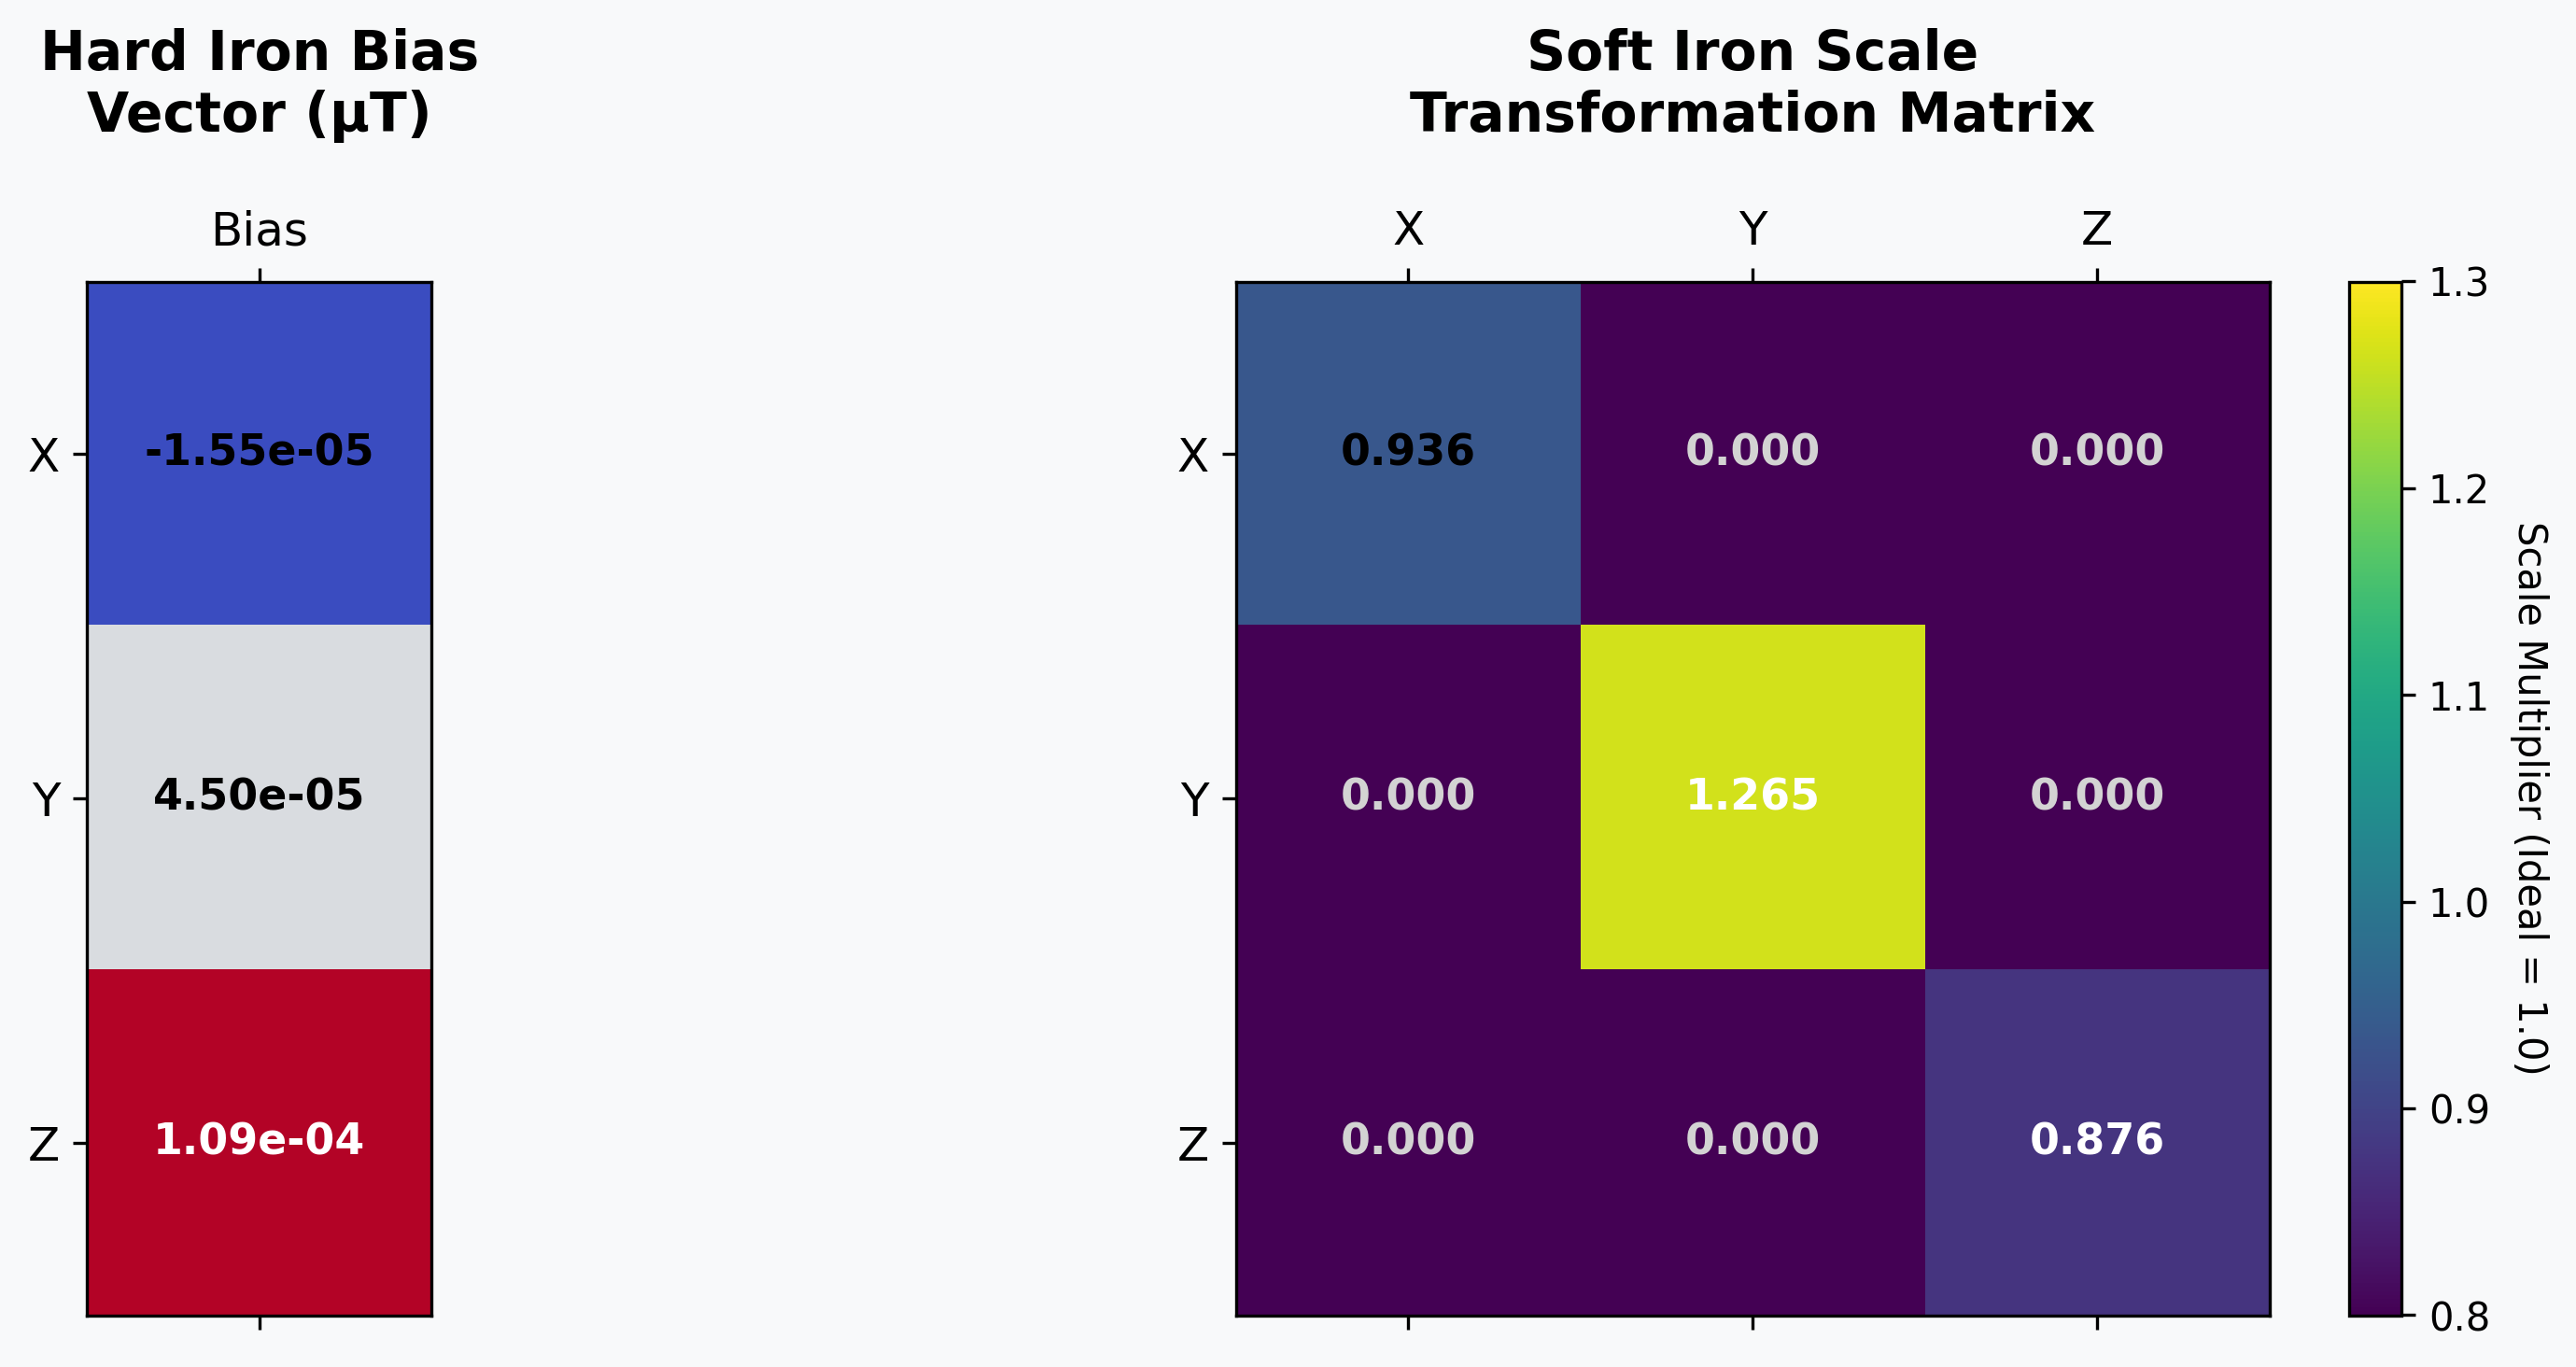
\includegraphics[width=0.5\linewidth]{mag_matrices_cmap.png}
    \caption{Hard-Iron and Soft-Iron Baises}
    \label{fig:placeholder}
\end{figure}

\section{Observations}

Here the performance of all five algorithms are compared. First all algorithms are compared when resting to visualize noise and drift when undisturbed.

\begin{figure}
    \centering
    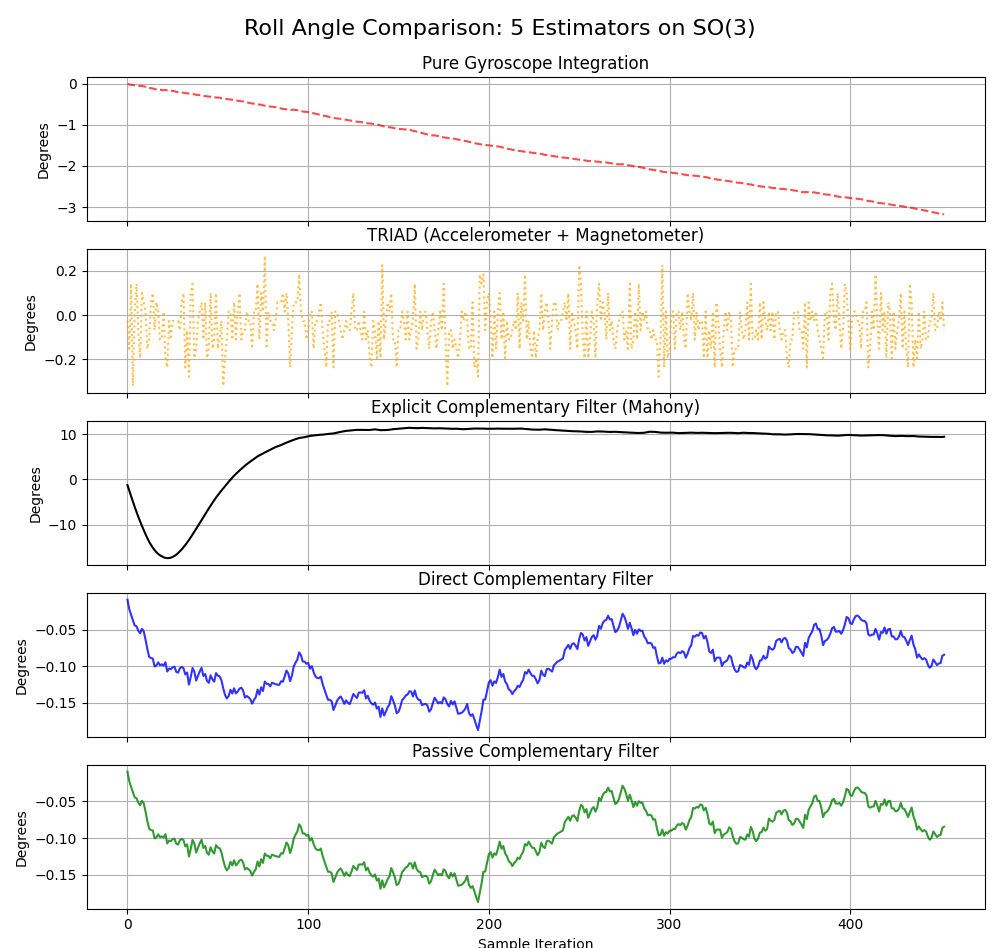
\includegraphics[width=0.9\linewidth]{resting_declination.png}
    \caption{Sensors at Rest}
    \label{fig:rest}
\end{figure}

Two immediate takeaways from Fig. \ref{fig:rest} come from

\begin{itemize}
    \item Pure Gyroscope Integration: Visible drift over time.
    \item Explicit Mahony Filter: Visible magnetic dip, resting above $0^\circ$. 
\end{itemize}

The rest of the algorithms provide an accurate representation of the roll angle over time. The drift from pure gyroscope integration is expected. The more curious result is the 10 degree deviation in the Mahony filter.\\
\\
\textbf{Magnetic Dip} is a phenomenon where Earth's True North (along the axis) deviates from directional North. According to the National Centers for Environmental Information, the dip expected at the latitude and longitude of measurement is $\sim 9.93 ^\circ$. This matches the observation in Fig. \ref{fig:rest}.\\
\\
One may expect to see the same phenomenon in the TRIAD algorithm too, since this too is reliant on magnetometer readings. However, since the second axis $t_2$ is computed as a cross product of the magnetic North vector and the gravitational reference vector, $t_2$ retains no information along the Z axis, completely ignoring the magnetic dip.

\subsection{Recorded Video}
This section refers to the video submitted along with this report.\\
\\
\begin{itemize}
    \item \textbf{Pure Gyroscope Integration (Compounding Error):}  While pure gyroscope tracks rapid rotations smoothly, its estimate \textbf{gradually drifts} away from the true orientation over time. This is because the gyroscope operates strictly open-loop. The discrete integration that converts angular velocities to angles does not have any absolute reference bounds.
    
    \item \textbf{TRIAD Algorithm (High-Frequency Jitter):} In the video, the TRIAD estimate successfully prevents long-term drift but exhibits violent, \textbf{high-frequency jitter} during dynamic movements. This is because the TRIAD algorithm is a memoryless estimator. It has no low-pass filtering or time history, any translational artifacts present themselves as sudden bumps and jitters.
    
    \item \textbf{Explicit Mahony Filter:} The Explicit filter successfully rejects the TRIAD jitter but appears to physically lag behind the actual rapid movements of the sensor. This can be attributed to the PI controller used by the filter to suppress noise. In order to filter out noise from the accelerometer, the proportional gain forces the system to act as a low pass filter. During dynamic, rapid rotations, the system can take some time to pull the estimate to the true orientation. There is a visible temporal \textbf{phase lag}. 
    
    \item \textbf{Direct and Passive Filters:} The direct and passive filters provide robust visual performance, perfectly tracking rapid movements without jitter, lag or drift. This can be attributed to the decoupled architecture that these filters are reliant on.\\
    \\
    The gyroscope is used as the primary engine, thus eliminating the jitter from the TRIAD algorithm and the lag from the Mahony filter. However, since the TRIAD matrix is used to compute the exact rotational error natively on the $SO(3)$ manifold, these algorithms can utilize a geometric anchor to correct for gyroscope errors. This prevents the drift of the pure gyroscopic algorithm.\\
    \\
    This results in high-frequency reliability of the gyroscope with the low-frequency absolute accuracy of the geometric anchoring vectors.
\end{itemize}

\begin{figure}
    \centering
    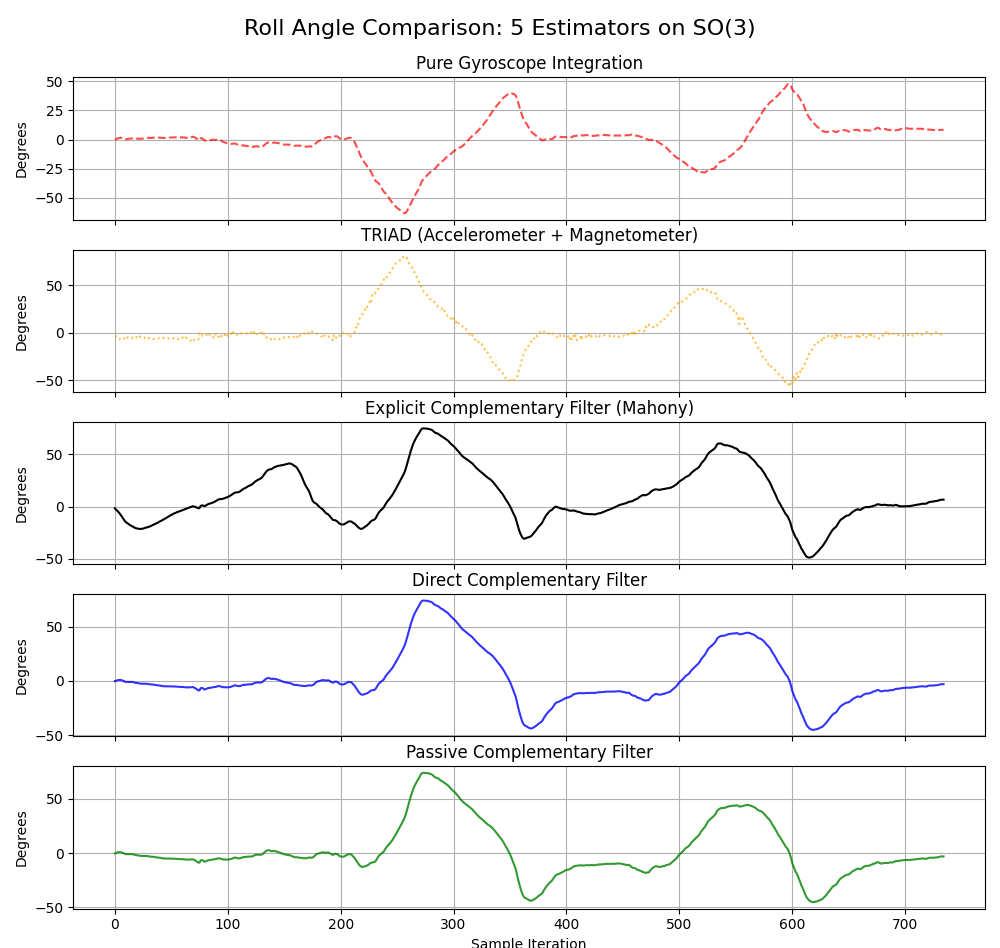
\includegraphics[width=0.8\linewidth]{recording1.png}
    \caption{Roll Angle -- Movement from the recording}
    \label{fig:recording1}
\end{figure}

% Needs an appendix

\end{document}
